Before discussing the results, first we have to formulate what we want to learn from this kind of generalisation. 
The main difference form previous literatuee was the use of transition to excited states before ionisation. 
In principle we want to investigate how this tranistion influeces the ionisation process or in general the ionisation rate.\\
Previously: time reversal symmetry, what causes it? \\
Also we want to know what influences the ionization rate more, the stark shift or the distortion of the ground state or the possibility for the electron to also get excited to higher states instead of direct ionization.\\
So lets start with the star effect.

\section{Stark Shift}
The Stark effect is the shift of the energy levels of an atom or molecule due to the presence of an external electric field.

\begin{figure}[H]
    \centering
    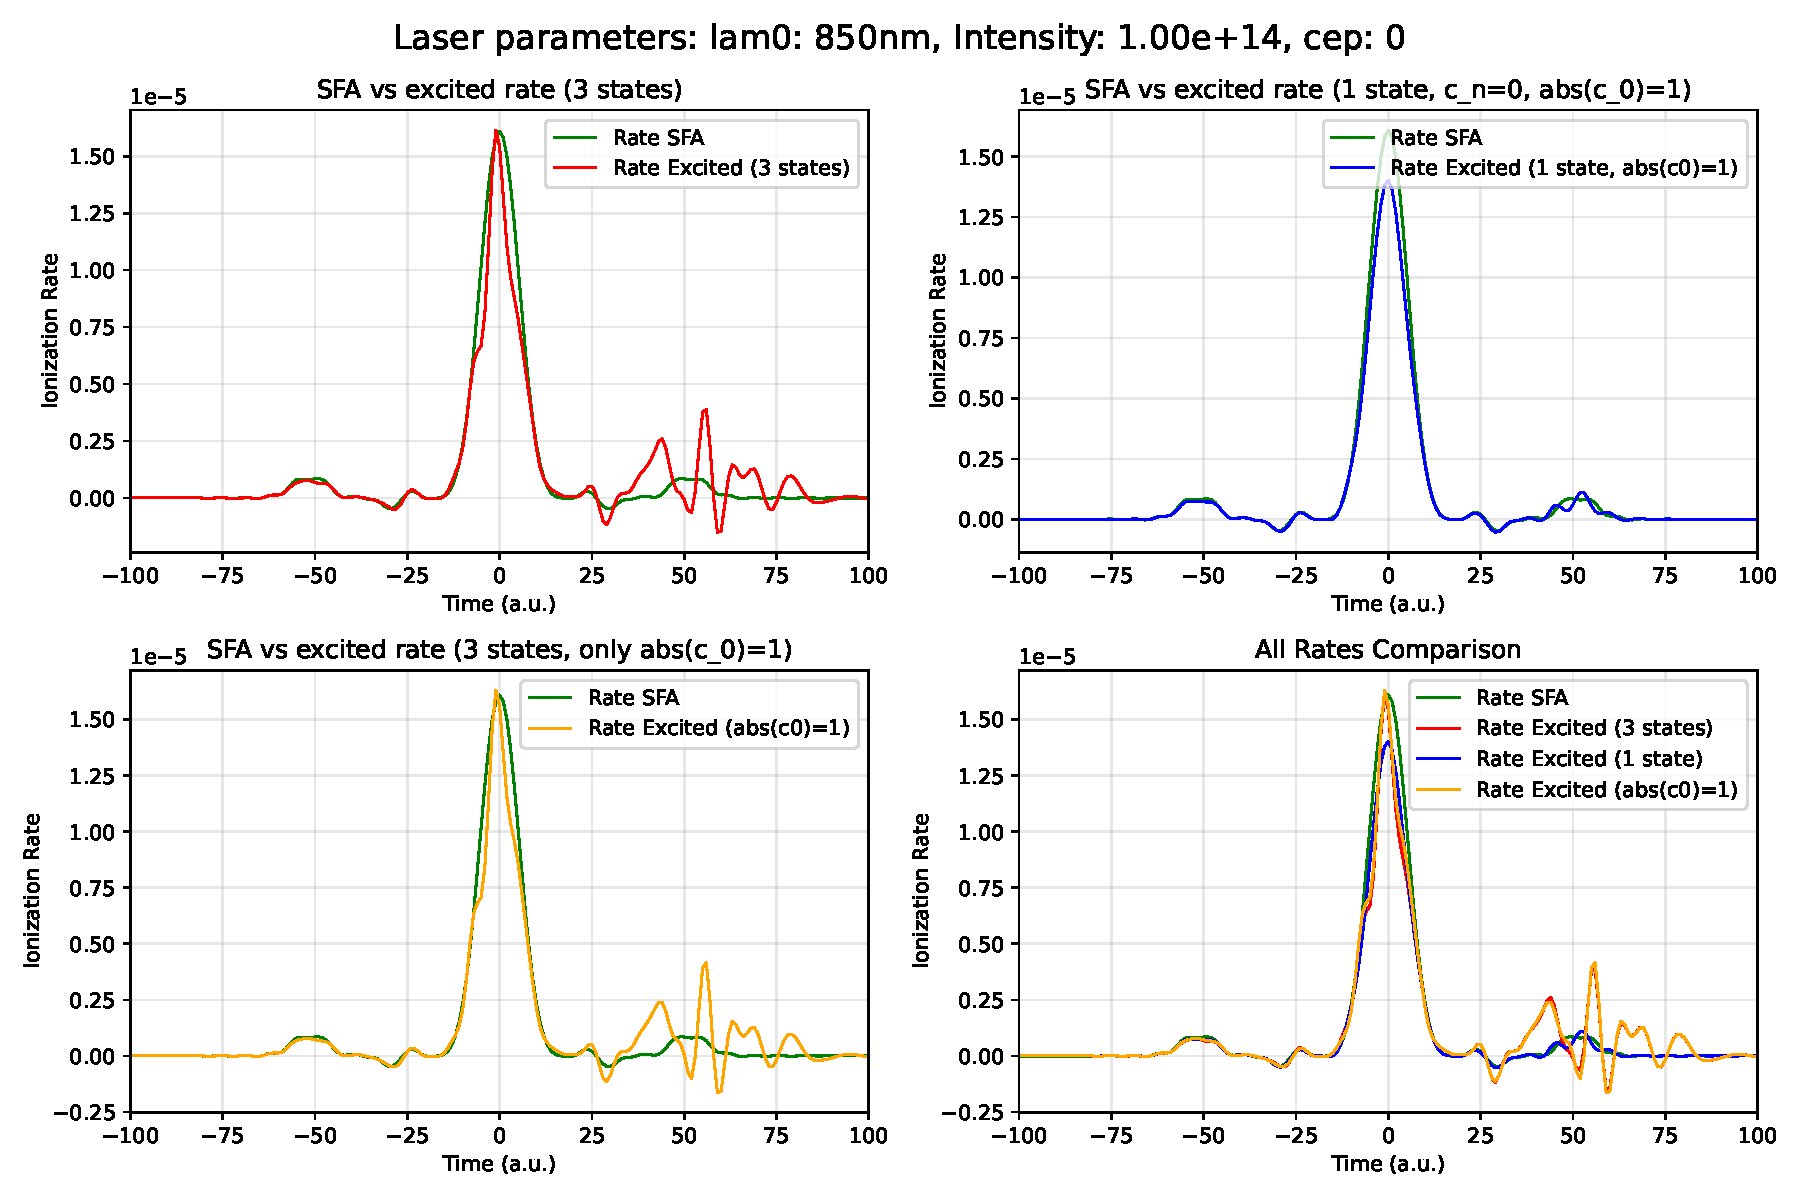
\includegraphics[width=0.9\textwidth]{figures/rate4_850_1.00e+14_onlystark.pdf}
    \caption{Sine function}
    \label{fig:starkeffect}
\end{figure}

Naiv: Stark effect changes energy in electron so its "harder" to ionise, thats why blue curve goes down (when excitedStates=1). 
But thats not certainly the case because of stark effect, thats why only set absc0 to 1 and phase remains. 
Example with oszillations with time dependent resonance frequency, and external force not at resonance but coincidence with oszillator resonance frequency so this may cause it.



%%%%%%%%%%%%%%%%%%%%
\section{Interpretation}
Stark shift doesnt seem to have much contribution (sadly).\\
Lets investigate the influence of first coefficient, nothing more. Only the phase has a contribution, the amplitude is not important.
It has a influence because 


%%%%%%%%%%%%%%%%
\section{Lorem}
This might be how it is supposed to be -- we are in the regime where the laser field is strong enough to ionize the atom, 
but we artificially force the electron to stay in the part of the Hilbert space covered by a few bound states. 
If the calculations are converged with respect to the time step, and you see convergence regarding the number of bound states in the weak-field regime, 
then it's fine if there is no convergence with respect to the number of bound states in the strong-field regime.




% \section{Laser Fields}
% Lorem ipsum dolor sit amet, consetetur sadipscing elitr, sed diam nonumy eirmod tempor invidunt ut labore et dolore magna aliquyam erat, sed diam voluptua. At vero eos et accusam et justo duo dolores et ea rebum. Stet clita kasd gubergren, no sea takimata sanctus est Lorem ipsum dolor sit amet. Lorem ipsum dolor sit amet, consetetur sadipscing elitr, sed diam nonumy eirmod tempor invidunt ut labore et dolore magna aliquyam erat, sed diam voluptua. At vero eos et accusam et justo duo dolores et ea rebum. Stet clita kasd gubergren, no sea takimata sanctus est Lorem ipsum dolor sit amet.


% \begin{equation}
%     \partial_t u = \mathcal{H}(t)  \lambda 
% \end{equation}

% \begin{figure}[H]
%     \centering
%     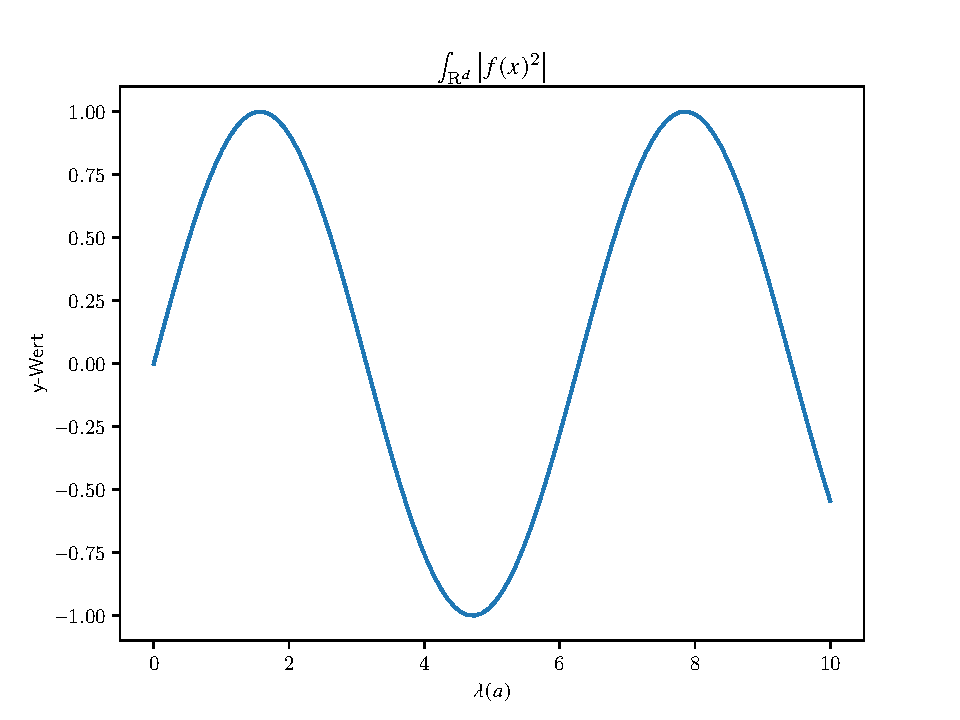
\includegraphics[width=0.5\textwidth]{figures/plot.pdf}
%     \caption{Sine function}
%     \label{fig:sinus}
% \end{figure}



% \begin{equation*}
%     \partial \A = \B
% \end{equation*}

% \medskip

% \begin{equation}
%     \int_{\R^d} \abs{f(x)}^2 \dd x = \int_{\R^d} \abs{\F f(\xi)}^2 \dd \xi
% \end{equation}

% \medskip

% \begin{equation}
%     %schrödinger equation
%     \ii \partial_t u = \mathcal{H}(t) \Ket{a} \lambda 
% \end{equation}

% \begin{equation}
%     \gimel \overrightarrow{a} \cos \mathrm{cos} \Rightarrow \Longrightarrow \nearrow 
% \end{equation}
